%!TEX root = ../dissertation.tex

\hypertarget{(chap:capitolo4)}{}
\chapter{Teoria sistemi di raccomandazione}
\section{Il problema}
Uno dei campi più popolari al momento verso cui si rivolge una particolare attenzione è quello dei sistemi di raccomandazione, in quanto l'attività online sta aumentando sempre più e nascono sempre più spesso nuovi servizi che permettono di scegliere oggetti, siano questi prodotti, video, musica, film o molto altro, da cataloghi vastissimi. I sistemi di raccomandazione permettono di navigare questi cataloghi andando a cercare gli oggetti che risultino più interessanti per l'utente. Definiamo i cosidetti "attori" del problema, gli user, ossia gli utenti del sistema, e gli item, ossia gli oggetti che si vuole consigliare. L'obiettivo del sistema può essere quello di consigliare ad uno user una lista di K item che si ritiene possano interessargli, oppure dato un item si può trovare una lista di item che si considerino simili allo stesso.
\section{Preliminari}
Abbiamo quindi due insiemi:
\begin{itemize}
	\item Users: insieme degli utenti di cui abbiamo informazioni;
	\item Items: insieme degli oggetti di cui abbiamo informazioni;
\end{itemize}
Solitamente le informazioni che si hanno a disposizione sono delle valutazione da parte dello user sull'item, queste possono essere di due tipi:
\begin{itemize}
	\item Implicito: 1 se l'utente ha espresso un qualche interesse per l'item, 0 se non c'è stata interazione;
	\item Esplicito: valutazione basata su una scala da 1 a N, 0 se c'è stata interazione;
\end{itemize}
\section{User-item matrix}
\begin{minipage}[H]{0.6\textwidth}
	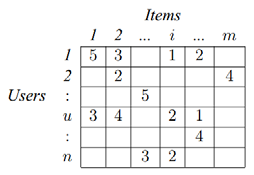
\includegraphics[width=7cm]{figures/Sample-of-user-item-matrix}
\end{minipage}
\begin{minipage}[H]{0.4\textwidth}
	bau
\end{minipage}